\chapter{The Large Hadron Collider}
%\section{Siliziumdetektoren}
The LHC was build between 1998 and 2008 by the European Organization for Nuclear Research (CERN) in collaboration with 10000 scientist from over 100 countries
and lies in a $\SI{27}{\kilo\meter}$ tunnel 175 metres underground in Switzerland near Geneva. It is a proton-proton synchrotron, which uses
the systems to accelerate the protons before they are injected into the main accelerator. The linear particle accelerator LINAC 4 generates $\SI{160}{\mega\eV}$
negative hydrogen ions and launches them into the Proton Synchrotron Booster (PSB). Here, the electrons are removed from the hydrogen ions, leaving only the nucleus
consisting of one proton, which then enters the Super Proton Synchrotron (SPS). It increases the protons energy to $\SI{450}{\GeV}$ and feeds them to the
LHC, where to opposing proton beams are accelerated. In the main ring,
the protons are accumulated to bunches and accelerated to their maximum energy of $\SI{13}{\tera\eV}$ in 20 minutes.

At four locations, the two proton beams
are crossed, making it possible for them to collide. Around these interaction points, the four large experiments, ATLAS, CMS, LHCb and Alice are operated.
Occasionaly lead nuclei are accelerated to study matter under extreme conditions at the ALICE experiment. The ATLAS and CMS experiment are general-purpose detectors for
high energy physics. They differ on their technical design to achieve their goal and enable to corrobate each others results.
LHCb is an asymmetric particle detector specialized in measuring the parameters of CP violation in B-meson decays.
Further experiments at the LHC include TOTem, LHCf, MoEDAL and FASER, which focus on specialized research. Figure \ref{fig:lhc_aufbau} shows a schematic depiction
of the LHC.

\begin{figure}[H]
  \centering
  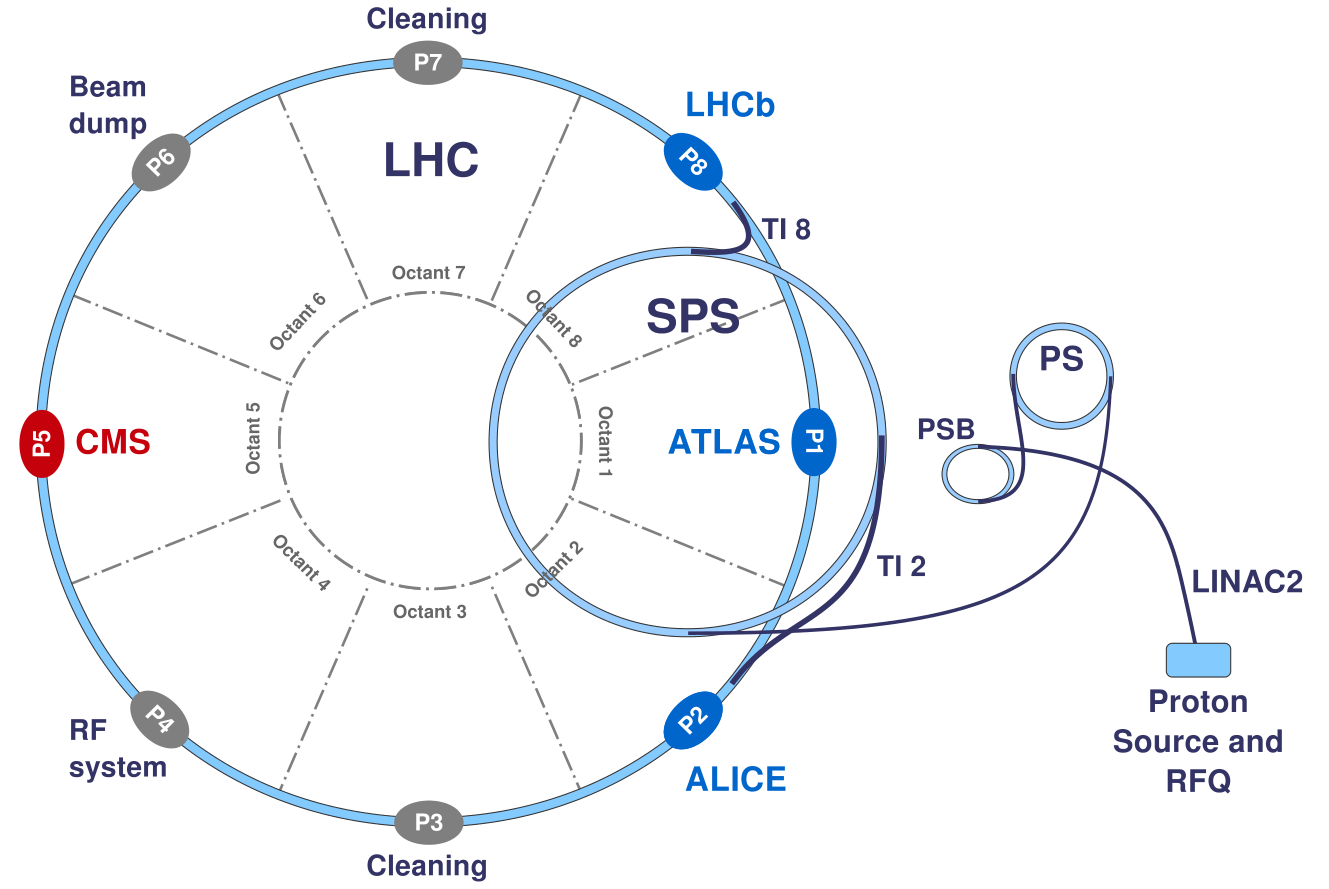
\includegraphics[height=0.4\textwidth]{images/lhc_aufbau.png}
  \caption{Schematic representation of the CERN accelerator complex (not to scale)\cite{lhc_aufbau}.}
  \label{fig:lhc_aufbau}
\end{figure}

After the second run from 2015 to 2018 followed the Long Shutdown 2 (LS2) until 2021 in order to upgrade the accelerator. The goal is to increase the luminosity by a factor of 10 by
implementing High Luminosity Large Hadron Collider (HL-LHC) in the Long Shutdown 3 (LS3), which is planned to be operational in 2026. Figure \ref{fig:lhc_plan} shows the timeline
of LHC programme.

\begin{figure}
  \centering
  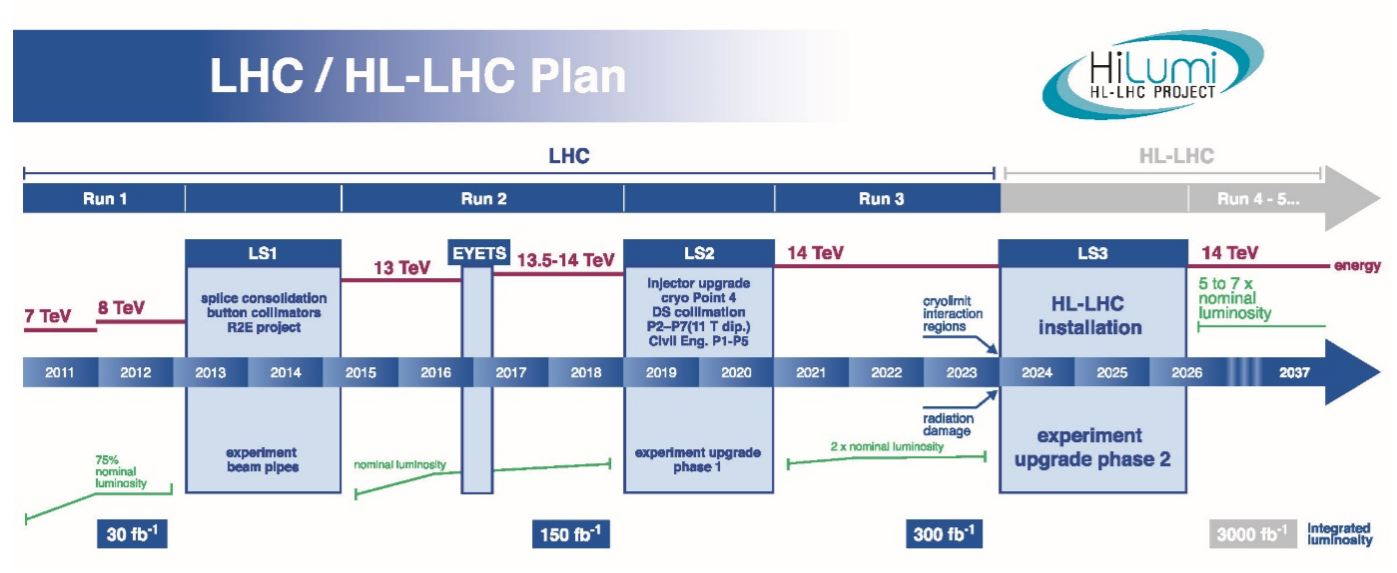
\includegraphics[height=0.4\textwidth]{images/lhc_plan.png}
  \caption{Timeline of the operational phases and Shutdowns of the LHC. The energy of accelerated protons in each phase is shown in red and the luminosity in green \cite{lhc_plan}.}
  \label{fig:lhc_plan}
\end{figure}

\section{The ATLAS detector}
The ATLAS detector is the largest general-purpose detector with a length of $\SI{46}{\meter}$ and a diameter of $\SI{25}{\meter}$.
It was designed to be a cylindric $4\pi$ detector, covering up most of the solid angle to detect particles flying in all directions.
Both ATLAS and CMS detected the Higgs Boson in 2012 and thus prove the existence of the last missing particle of the standard model.
Further goals of the detector is to search for beyond the standard model physics in the high energy domain, where current theories possibly break down.
Top quarks, which were produced at the LHC in large amount of quantities for the first time, can be studied more precisely with the help of the ATLAS detector.

The entire detector is made out of four different layers of detector systems, the Inner Detector, the electromagnetic and hadronic calorimeters
and the muon spectrometer. Only a couple of centimeter away from the interaction point lies the Inner Detector with its purpose to track the produced charged particles.
It is made of three subsequent components, with the innermost layer called the Pixel Detector and consists of three layers of silicon pixel detectors. The middle constituent
is the Semiconductor Tracker (SRT) with a similar purpose. Here, four layers of silicon stripe detectors are used for detection, while they have a lower spatial resolution, a larger
area can be covered with them more efficiently. The Transition Radiation Tracker (TRT) is the outermost component and uses straw detectors for tracking as well as materials with
different refractive index inbetween the straws. Relativistic particles will produce transition radiation by traversing these materials, which enables particle
identification, especially for light charged particles.
A magnetic solenoid surrounding the Inner Detector produces a $\SI{2}{\tesla}$ magnetic field to curve the trajectories of charged particles in order to determine their
momentum. \\
The electromagnetic calorimeter is positioned outside the magnetic field and aims at absorbing electrons, positrons and photon induced
electromagnetic showers in order to measure the energy of the initial particle. Lead and stainless steel serve as the energy absorbing material and liquid argon as the
sampling material. Hadrons tend to traverse the electromagnetic calorimeter without losing all their energy, which is the reason the hadronic calorimeter comes after.
It uses steel as sampling material and scintillating tiles to measure the energy. \\
Because muons easily pass both calorimeters, the outermost detector system is the muon spectrometer consisting of silicon detectors to track the muons and three toroidal magnets
building up a magnetic field for momentum measurement. Figure \ref{fig:atlas} ilustrates the ATLAS detector with its components.

\begin{figure}
  \centering
  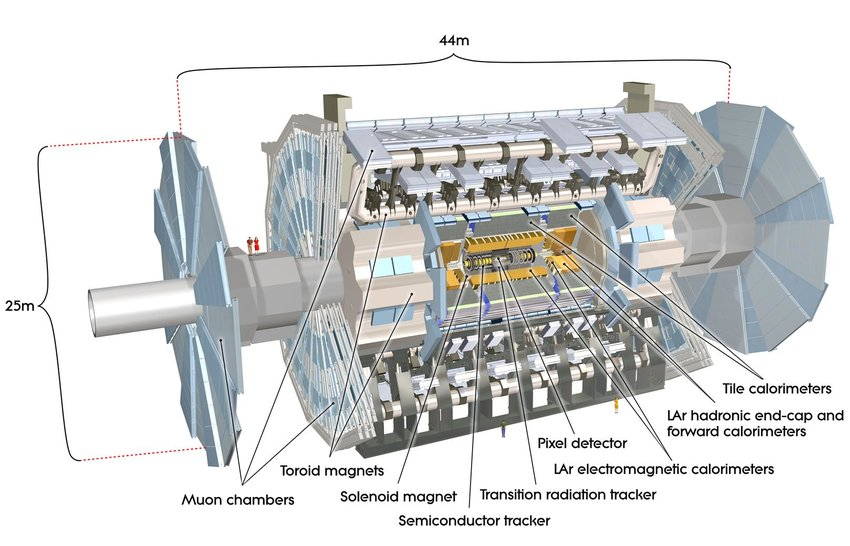
\includegraphics[height=0.5\textwidth]{images/atlas.png}
  \caption{Illustration of the ATLAS detector and its subsequent components. Two Humans are depicted at the bottom for a size comparison \cite{atlas}.}
  \label{fig:atlas}
\end{figure}

During the Long Shutdown 3 of the LHC, the ATLAS Inner Tracker (ITk) upgrade is planned to be installed. Its goal is to perform as good or better as the current detector, while
withstanding the harsher environment of the HL-LHC.

\chapter{Testbeam}
Studying the properties of sensor modules is crucial for an optimal performance of particle detectors. The new pixel modules used for the ATLAS ITk upgrade have to be thoroughly
tested in terms of efficiency and radiation hardness in order to fulfill the necessary requirements for their installment.
In order to evaluate the sensors performance they are irradiated in testbeam experiments similar to the conditions in the LHC.
These beam test measurements are performed mainly in two testbeam facilities, being located at Cern and Deutsches Elektronen Synchrotron (DESY). Sensors that are planned to be
installed in the ATLAS ITk are tested at DESY during the LS2.

\section{DESY Testbeam}
DESY is a national research center located at Hamburg. It operates the electron synchrotron DESY II since 1987 initially to accelerate electrons before injecting them into
HERA, the largest synchrotron at DESY. After the shut down of HERA in 2007, DESY II is now used for testbeam measurements. It produces an electron beam with energies upto
$\SI{7}{\GeV}$, which collides with a carbon fiber target creating bremsstrahlung in the process. The photons are extracted and collide with a secondary target
converting them to electron positron pairs. A dipole magnet behind the target creates a homogenous magnetic field to filter out unwanted energies and particles. This process
is shown schematically in figure \ref{fig:testbeam}.

\begin{figure}
  \centering
  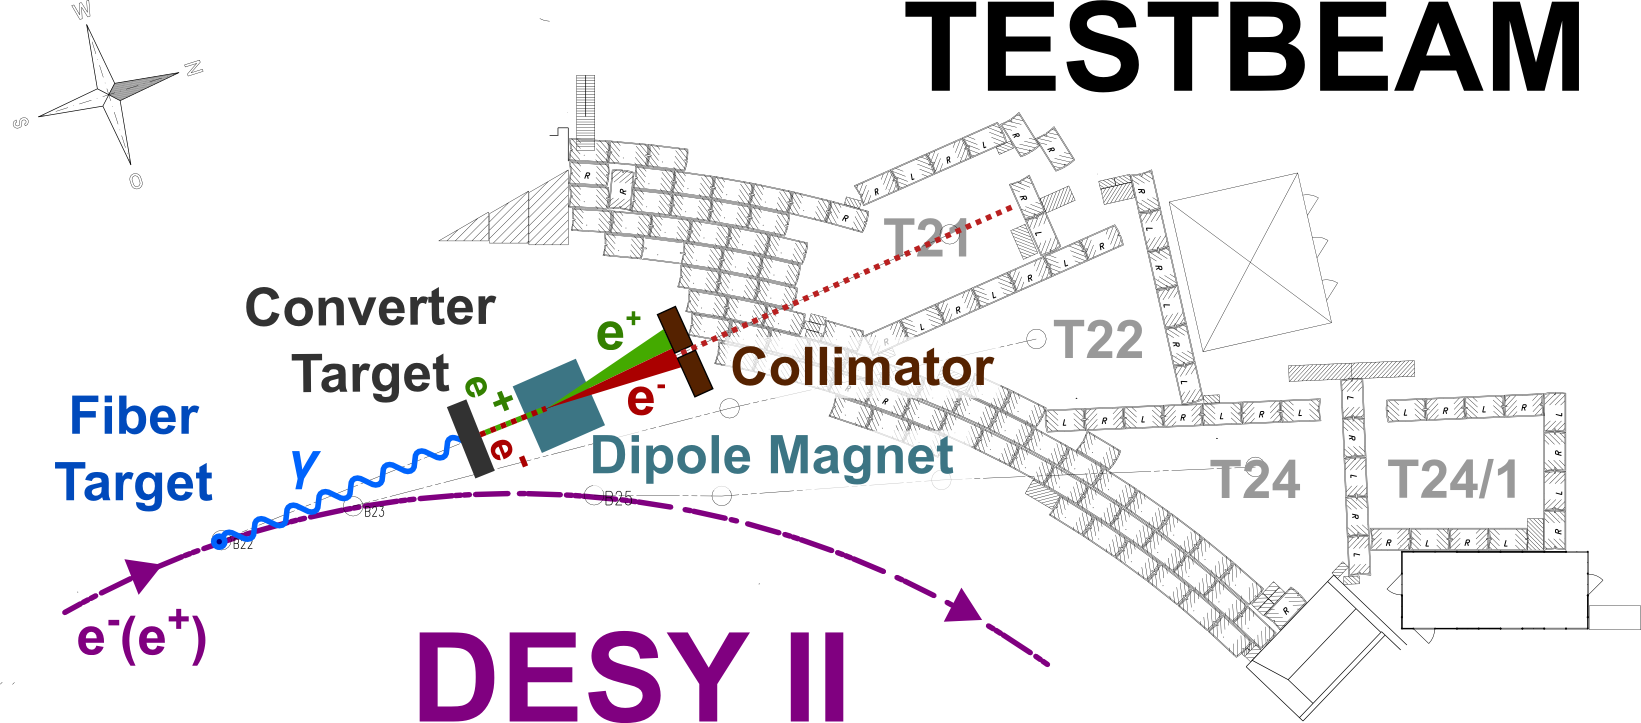
\includegraphics[height=0.4\textwidth]{images/desy.png}
  \caption{Depiction of the beam generation in testbeam experiments going through the beam line TB21 \cite{testbeam}.}
  \label{fig:testbeam}
\end{figure}

The permantly installed EUDET-type Pixel Beam telescopes DATURA and DURANTA are located behind the beam lines TB21 and TB22 and enable the tracking of the particles
produced by DESY II. Both telescopes consist of six Mimosa26 monolithic active pixel sensors with %a pixel pitch of $\SI{18.4}{\micro\meter} \times \SI{18.4}{\micro\meter}$.
three sensors each incorporated into one arm of the telescope and the DUT's being placed inbetween. A polystyrene box filled with dry ice is used to cool the DUT's to
avoid annealing and other unwanted effects due to heat. For time references during the measurements, an FE-I4 sensor is placed behind the telescope with a
time resolution of $\SI{25}{\nano\second}$ The sensors contain $336 \times 80$ pixels with a
$\SI{50}{\micro\meter} \times \SI{250}{\micro\meter}$ pixel pitch. Figure \ref{fig:telescope} shows the telescope setup of DATURA.

%\begin{figure}
%  \centering
%  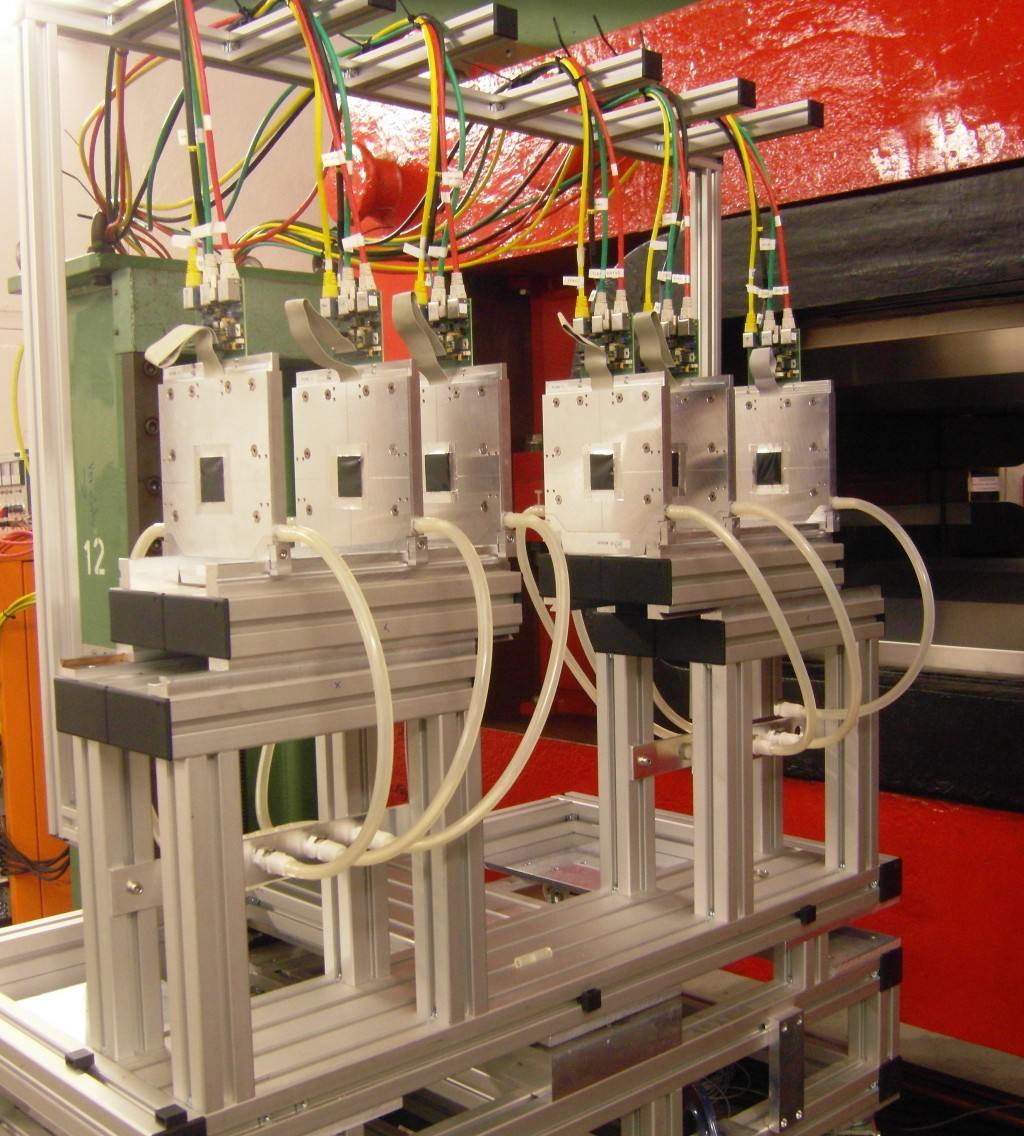
\includegraphics[height=0.4\textwidth]{images/telescope.jpg}
%  \caption{Shown is the Beam telescope DATURA consisting of six Mimosa26 sensors placed in the jigs. The tubes connected to the sensors transport water to
%  cool the sensors \cite{telescope}.}
%  \label{fig:telescope}
%\end{figure}

\begin{figure}
  %\centering
  \begin{subfigure}{0.48\textwidth}
      \centering
      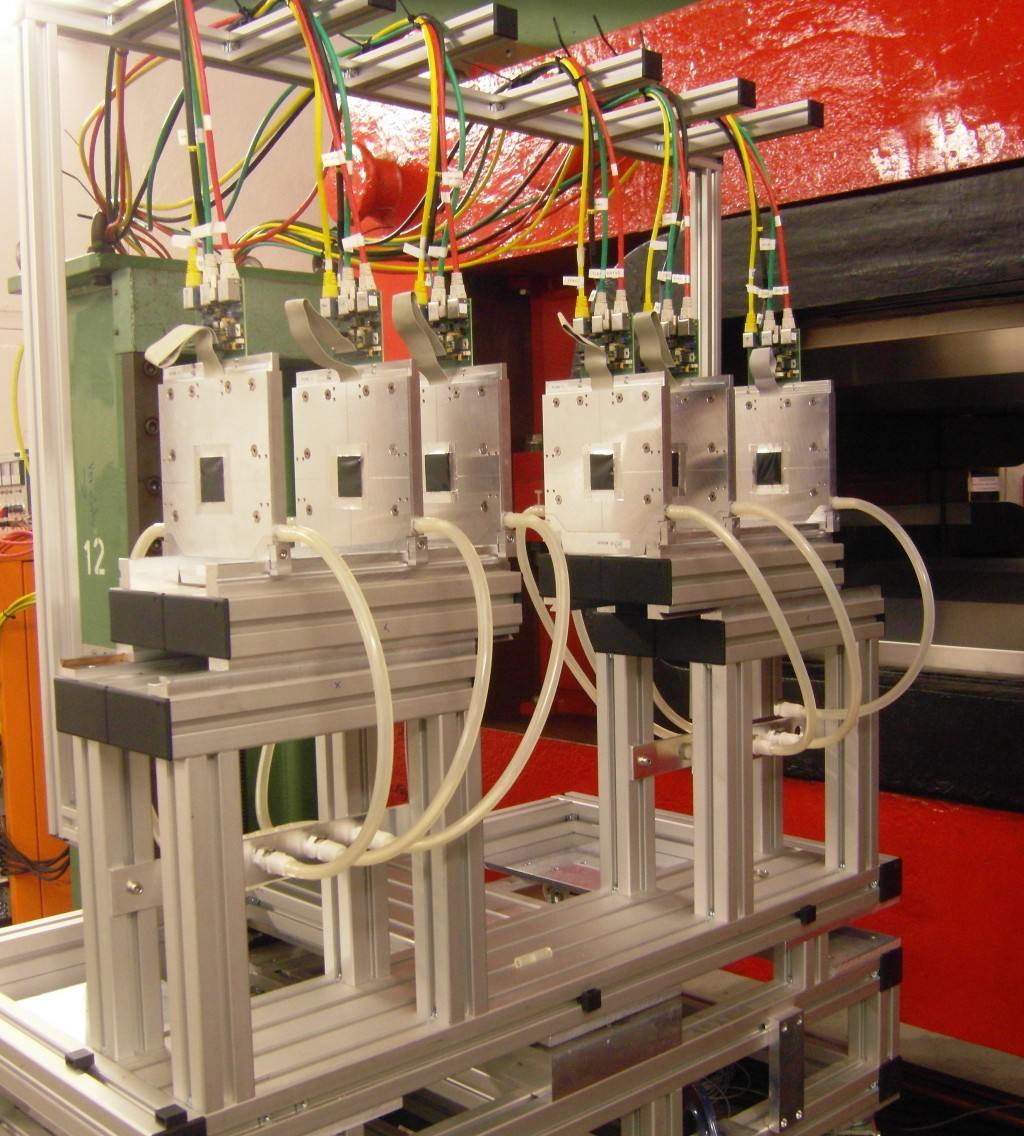
\includegraphics[height=0.82\textwidth]{images/telescope.jpg}
  \end{subfigure}
  \begin{subfigure}{0.48\textwidth}
      %\centering
      \hspace{-1cm}
      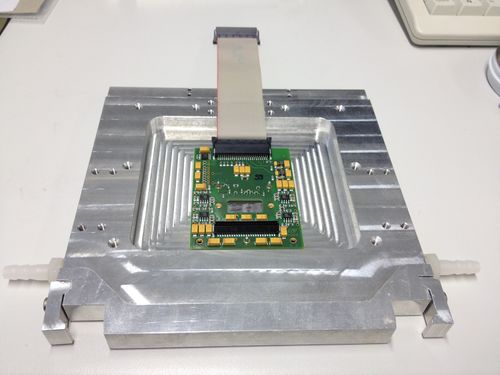
\includegraphics[height=0.82\textwidth]{images/mimosa.jpg}
  \end{subfigure}
  \caption{Shown on the left is the Beam telescope DATURA consisting of six Mimosa26 sensors placed in the jigs. The tubes connected to the sensors transport water to
  cool the sensors \cite{telescope}. Shown on the right is the Mimosa26 board inside the aluminium housing \cite{mimosa}. }
  \label{fig:telescope}
\end{figure}

Mimosa26 are fabricated in a standard $\SI{0.35}{\micro\meter}$ CMOS process with a fast binary read out
%size of $\SI{13.7}{\milli\meter} \times \SI{21.5}{\milli\meter}$.
Signals are measured with a time resolution of $\SI{230}{\micro\second}$ with each measurement in a read out cycle belonging to the same event.
They contain $576 \times 1152$ pixels with a pixel pitch of $\SI{18.4}{\micro\meter} \times \SI{18.4}{\micro\meter}$
and a thickness of $\SI{50}{\micro\meter}$.

The generic data aquisition framework EUDAQ records the data produced in testbeam experiments. Its centrally handles the data flow and synchronises data stream to enable
the integration of different independent devices under test. An exemplary setup of a beam telescope with EUDAQ is shown in figure \ref{fig:eudaq_bild}.
More information in \cite{eudaq}.

\begin{figure}
  \centering
  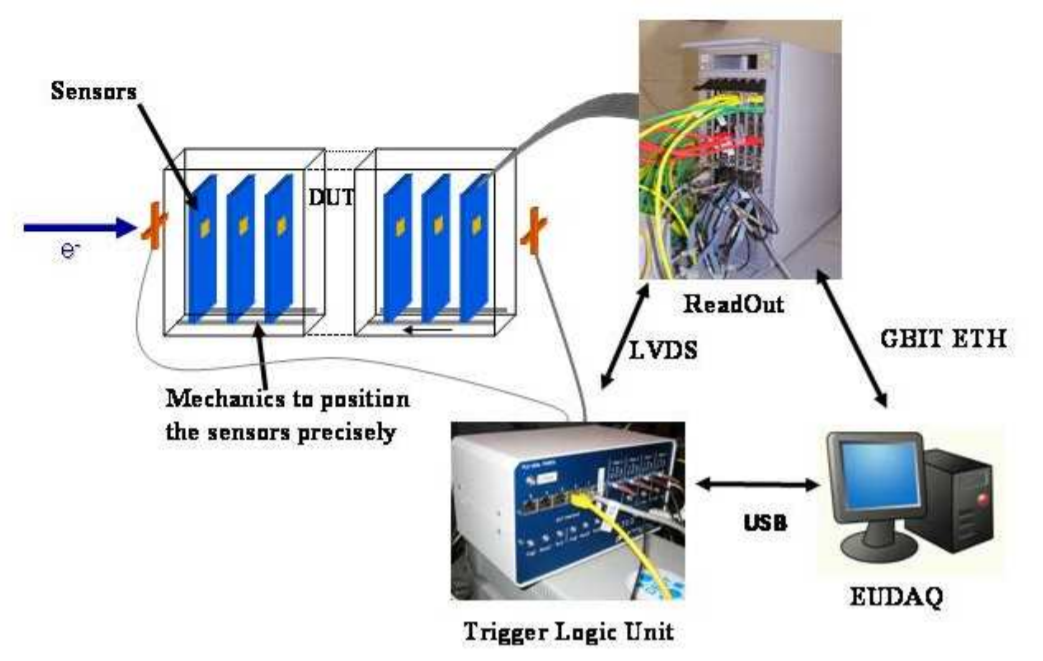
\includegraphics[height=0.4\textwidth]{images/eudaq.png}
  \caption{Necessary components for an analogue telescope \cite{eudaq_bild}.}
  \label{fig:eudaq_bild}
\end{figure}

\chapter{The track reconstruction framework EUTelescope}
The hit information of the sensor planes can be used to reconstruct the initial particles track. In order to do that the sotware EUTelescope was developed and
primarily used since 2007. It uses the Modular Analysis and Reconstruction for the Linear Collider (MARLIN) framework, which is part of the
International Collider Software package (ILCSoft). Each step in the reconstruction depends on MARLIN processors, which read in data, modifies and outputs new data to be
taken by the next processors. The individual steps in the reconstruction will call on certain processors specified for its task resulting in a
modular structure.

Information about the telescope geometry is stored in  Geometry API for Reconstruction (GEAR) files. This includes the position and rotation
of the sensors as well as their pixel layouts. Further parameters like radiation hardness, magnetic field and general properties of the used sensors have to be
specified to ensure proper track reconstruction.

General parameters and parameters in individual reconstruction steps are specified in the configuration file. This includes the import of the raw data and the
geometry file, the applied reconstruction steps and the definition of the cuts. \\
The steering files define the processors used in each reconstruction step and in which order they are executed.

A complete track reconstruction with EUTelescope contains the converter, the clustering, the hitmaker, the alignment and the track fitting in this respective order.
First, the raw data has to be converted to the lcio format for subsequent MARLIN processors. In addition, the module detects noisy pixels by analysing the
hit rate of the pixels and dividing them by the sum of measured events. The resulting firing frequency can be limited by user defined cuts, thus removing entries
from noise considered pixels from the lcio file.

In the clustering process, hit information on a sensor plane generated by the same particle will be clustered. Cluster with more than one pixel occur due
particles traversing through multiple pixels or charge sharing. Pixels will be grouped together based on their distance.
Regulation of the clustering process is then possible with cuts on the pixel distances.

The hitmaker step determines the particles hit position, the cluster center, of each cluster. For one pixel cluster, the cluster center is equal to the middle of
te pixel. Cluster centers of clusters with more than one pixel are calculated with a charge weighted center of gravity algorithm. This means, that
the deposited charge of each pixel is taken into account to derive the particles position. The cluster centers are transformed to the global coordinate
system of the telescope to function as the hit position for the track reconstruction. Global hit information on the sensors of particle tracks is assumed to be correlated with only
a small spread of the beam angle, which makes an initial guess of the telescope alignment, the prealignment, possible. 
